\subsection{Fase V: Lanzamiento}
En esta fase se realizó la puesta en producción de la aplicación web, móvil y el API junto al modelo analítico
de BI. Para la puesta en producción de la aplicación web y el API se utilizó Railway, un servicio de alojamiento de aplicaciones web que permite
desplegar aplicaciones de forma sencilla y rápida manejando el proceso de CI/CD al desplegar los sistemas desde su repositorio en GitHub, en las
Figuras \ref{fig:despliegue-web} y \ref{fig:despliegue-api} se muestran los servicios desplegados en Railway.

\begin{figure}[H]
    \centering
    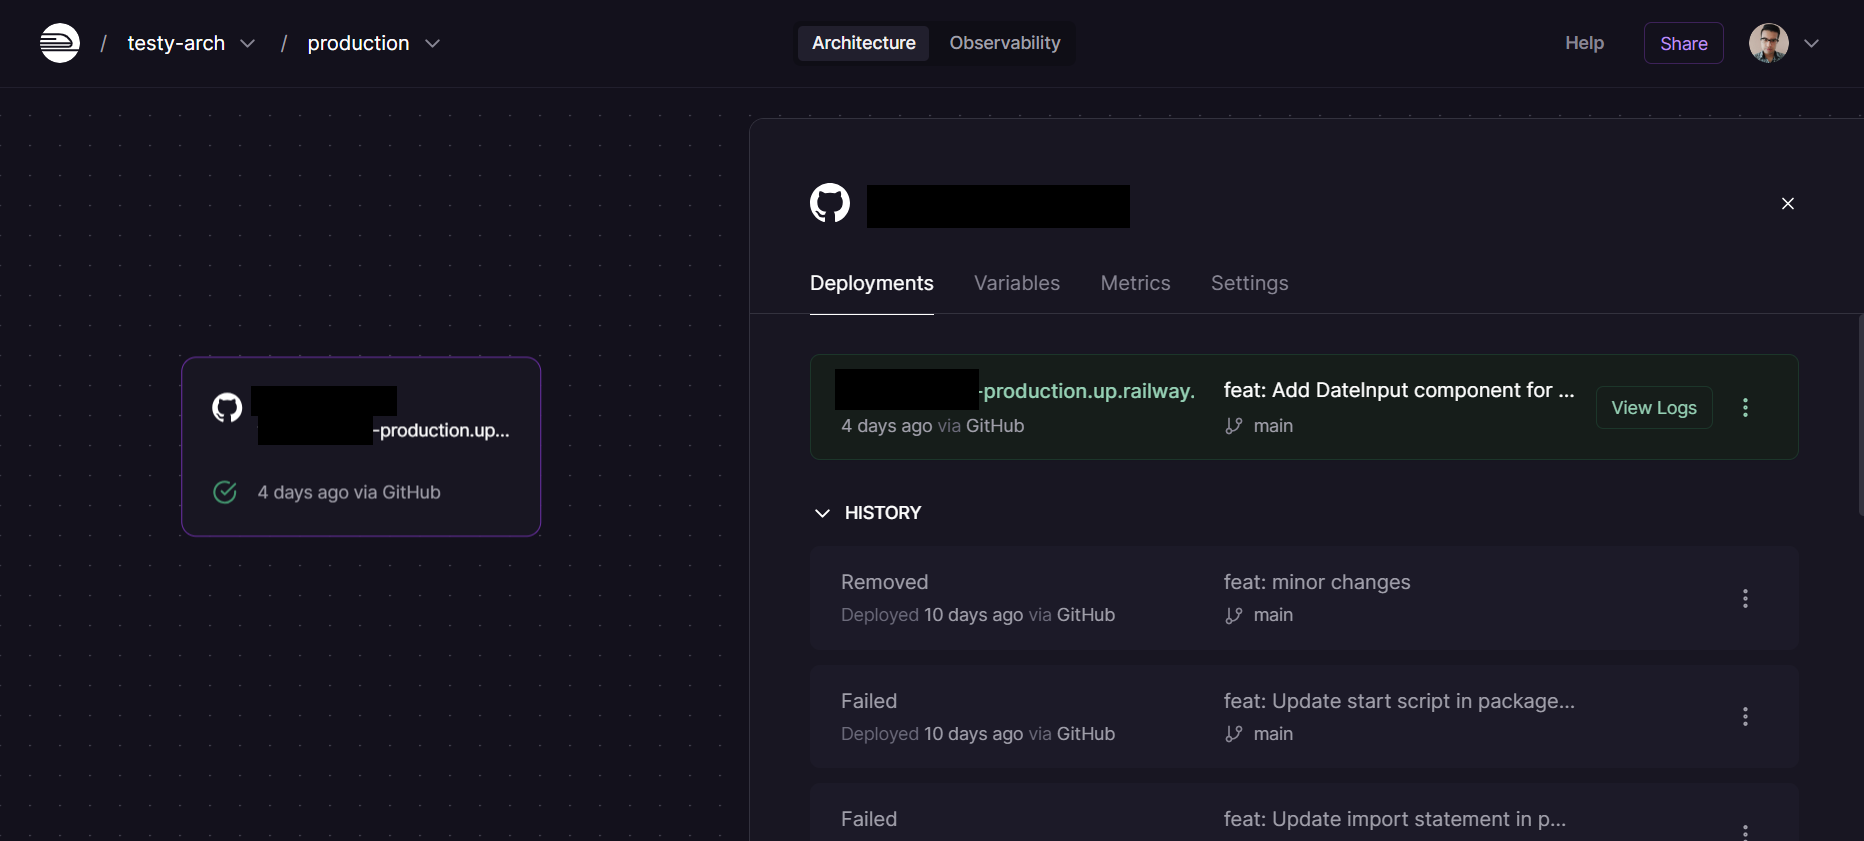
\includegraphics[width=0.8\textwidth]{chapters/III-resultados-y-discusion/resources/images/despliegue-web.png}
    \caption{Despliegue de la aplicación web en Railway.}
    \label{fig:despliegue-web}
\end{figure}

\begin{figure}[H]
    \centering
    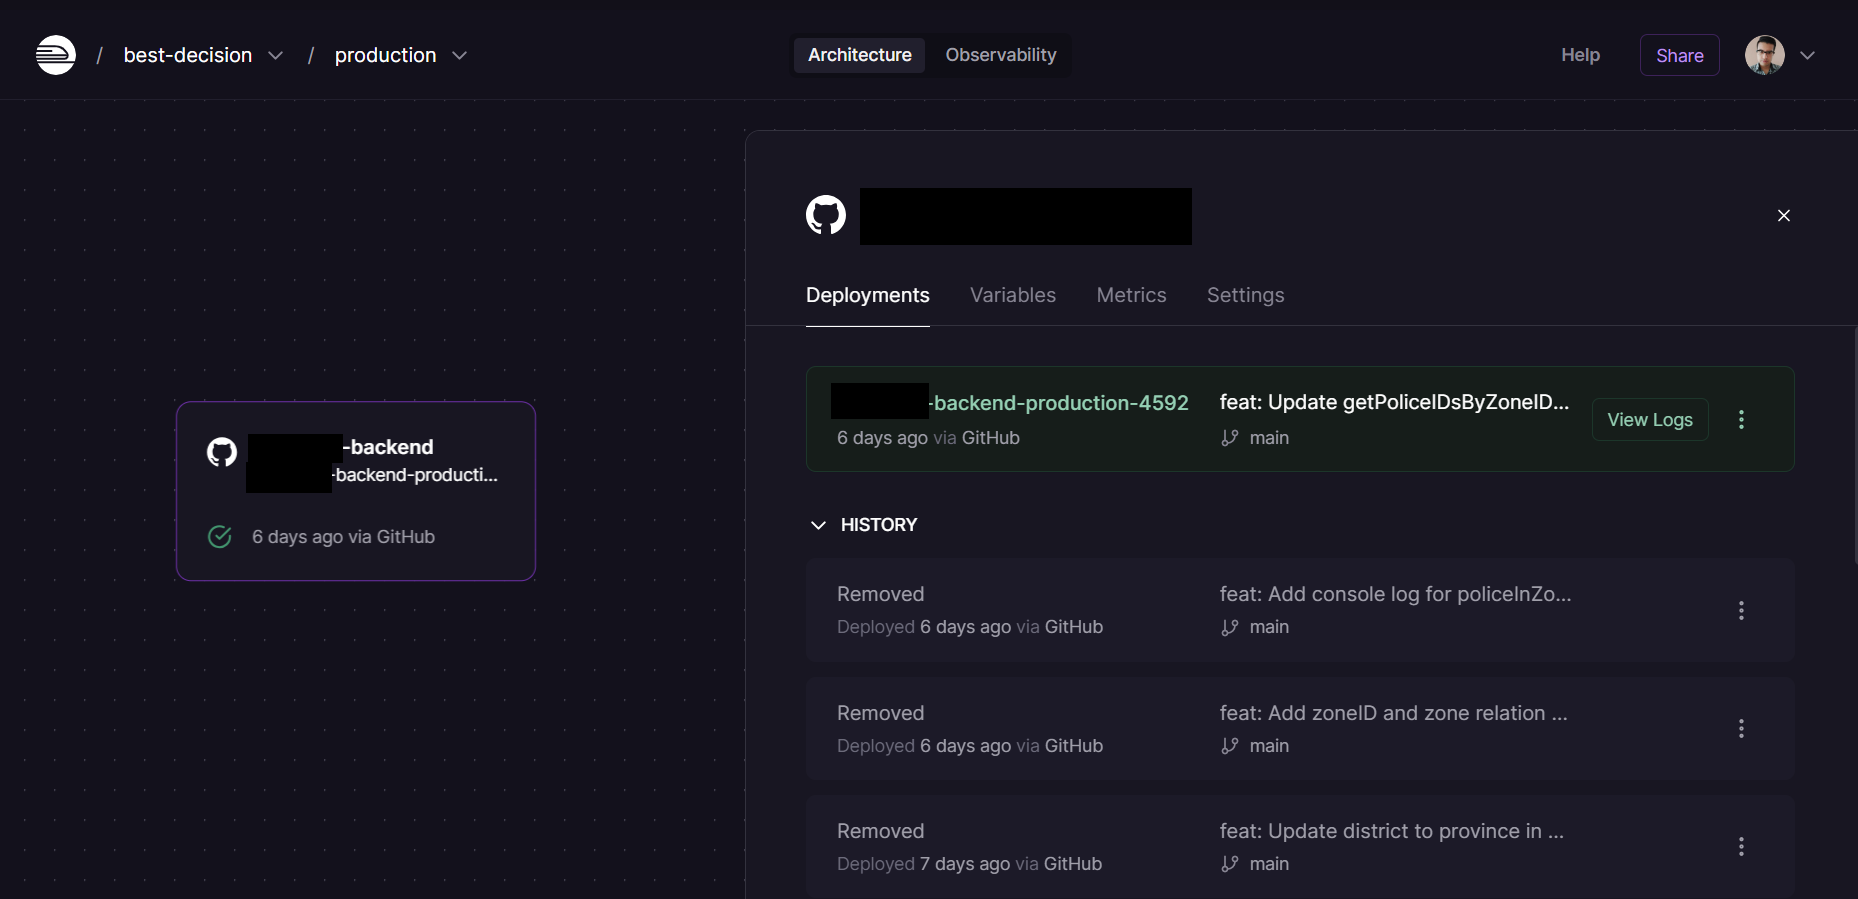
\includegraphics[width=0.8\textwidth]{chapters/III-resultados-y-discusion/resources/images/despliegue-api.png}
    \caption{Despliegue del API en Railway.}
    \label{fig:despliegue-api}
\end{figure}

Para la aplicación móvil se creo un archivo APK que permite instalar la aplicación en dispositivos Android, en la Figura \ref{fig:apk-movil}
se muestra el archivo APK generado para la aplicación móvil.

\begin{figure}[H]
    \centering
    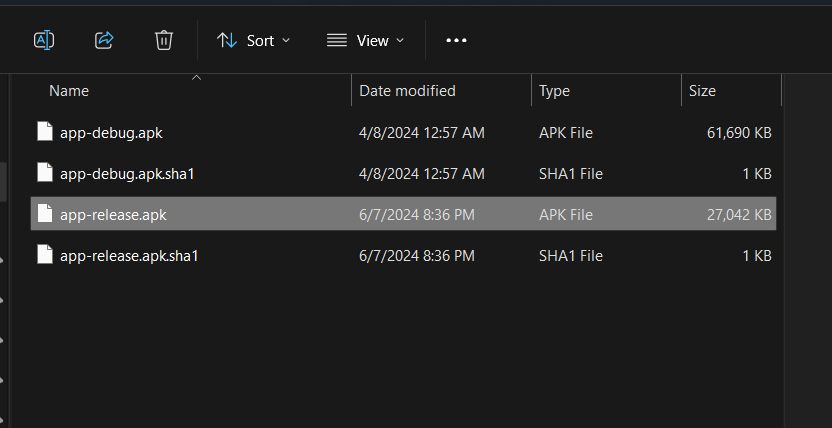
\includegraphics[width=0.8\textwidth]{chapters/III-resultados-y-discusion/resources/images/apk-movil.png}
    \caption{Archivo APK de la aplicación móvil.}
    \label{fig:apk-movil}
\end{figure}


Para la puesta en producción del modelo analítico de BI se lo mantuvo en el servidor de SQL Server Analysis Services de forma local, esto
debido a que no se contaba con un servidor de Analysis Services en la nube ni las licencias necesarias para obtener uno.
